\documentclass[12pt]{exam}
\usepackage[utf8]{inputenc}
\usepackage[swedish]{babel}
\usepackage{enumitem}
\usepackage{graphicx}
\usepackage{xcolor}
\usepackage{framed}

\pagestyle{headandfoot}
\header{\footnotesize Klass:\\Namn:}{\Large\textbf{Organisk kemi - Bedömningsanvisningar}\medskip}{\footnotesize Naturkunskap 2 - 2025}
\headrule
\footrule
\setlength{\columnsep}{0.25cm}
\footer{}{Sida \thepage}{Organisk kemi}

\newenvironment{answer}
  {\begin{framed}\color{blue}\textbf{Bedömning:} }
  {\end{framed}}

\begin{document}

\section*{Instruktioner}
Provet består av frågor av olika typer. Läs frågorna ordentligt innan du svarar.

\subsection*{Poäng}
Antalet poäng är markerat för varje fråga. Totalt \textbf{22 poäng}.\\ \textit{För godkänt krävs minst 10 poäng.}

\vspace{5mm}
\hrule

\begin{questions}

\question Ange vilka partiklar en atom består av och vilken laddning de har. (\textbf{1 poäng})
\vspace{5mm}

\begin{answer}
\textbf{Korrekt svar:} En atom består av:
\begin{itemize}
  \item Protoner (positiv laddning, +)
  \item Neutroner (neutral laddning, 0)
  \item Elektroner (negativ laddning, -)
\end{itemize}

\textbf{Poängbedömning:}
\begin{itemize}
  \item 1 poäng: Alla tre partiklar nämns med korrekt laddning
  \item 0 poäng: Ofullständigt svar eller felaktiga laddningar
\end{itemize}
\end{answer}
\vspace{5mm}

\question Förklara följande ord: (\textbf{1 poäng})
\begin{itemize}
  \item grundämne
  \item atomnummer
  \item masstal
\end{itemize}
\vspace{5mm}

\begin{answer}
\textbf{Korrekt svar:}
\begin{itemize}
  \item \textbf{Grundämne:} Ett ämne som består av endast en sorts atomer
  \item \textbf{Atomnummer:} Antalet protoner i atomkärnan (bestämmer vilket grundämne det är)
  \item \textbf{Masstal:} Summan av antalet protoner och neutroner i atomkärnan
\end{itemize}

\textbf{Poängbedömning:}
\begin{itemize}
  \item 1 poäng: Alla tre begrepp förklaras korrekt
  \item 0,5 poäng: Två begrepp förklaras korrekt
  \item 0 poäng: Endast ett eller inget begrepp förklaras korrekt
\end{itemize}
\end{answer}
\vspace{5mm}

\question Hur många valenselektroner har syre? Motivera utifrån bilden. (\textbf{1 poäng})

\begin{figure}[h]
  \centering
  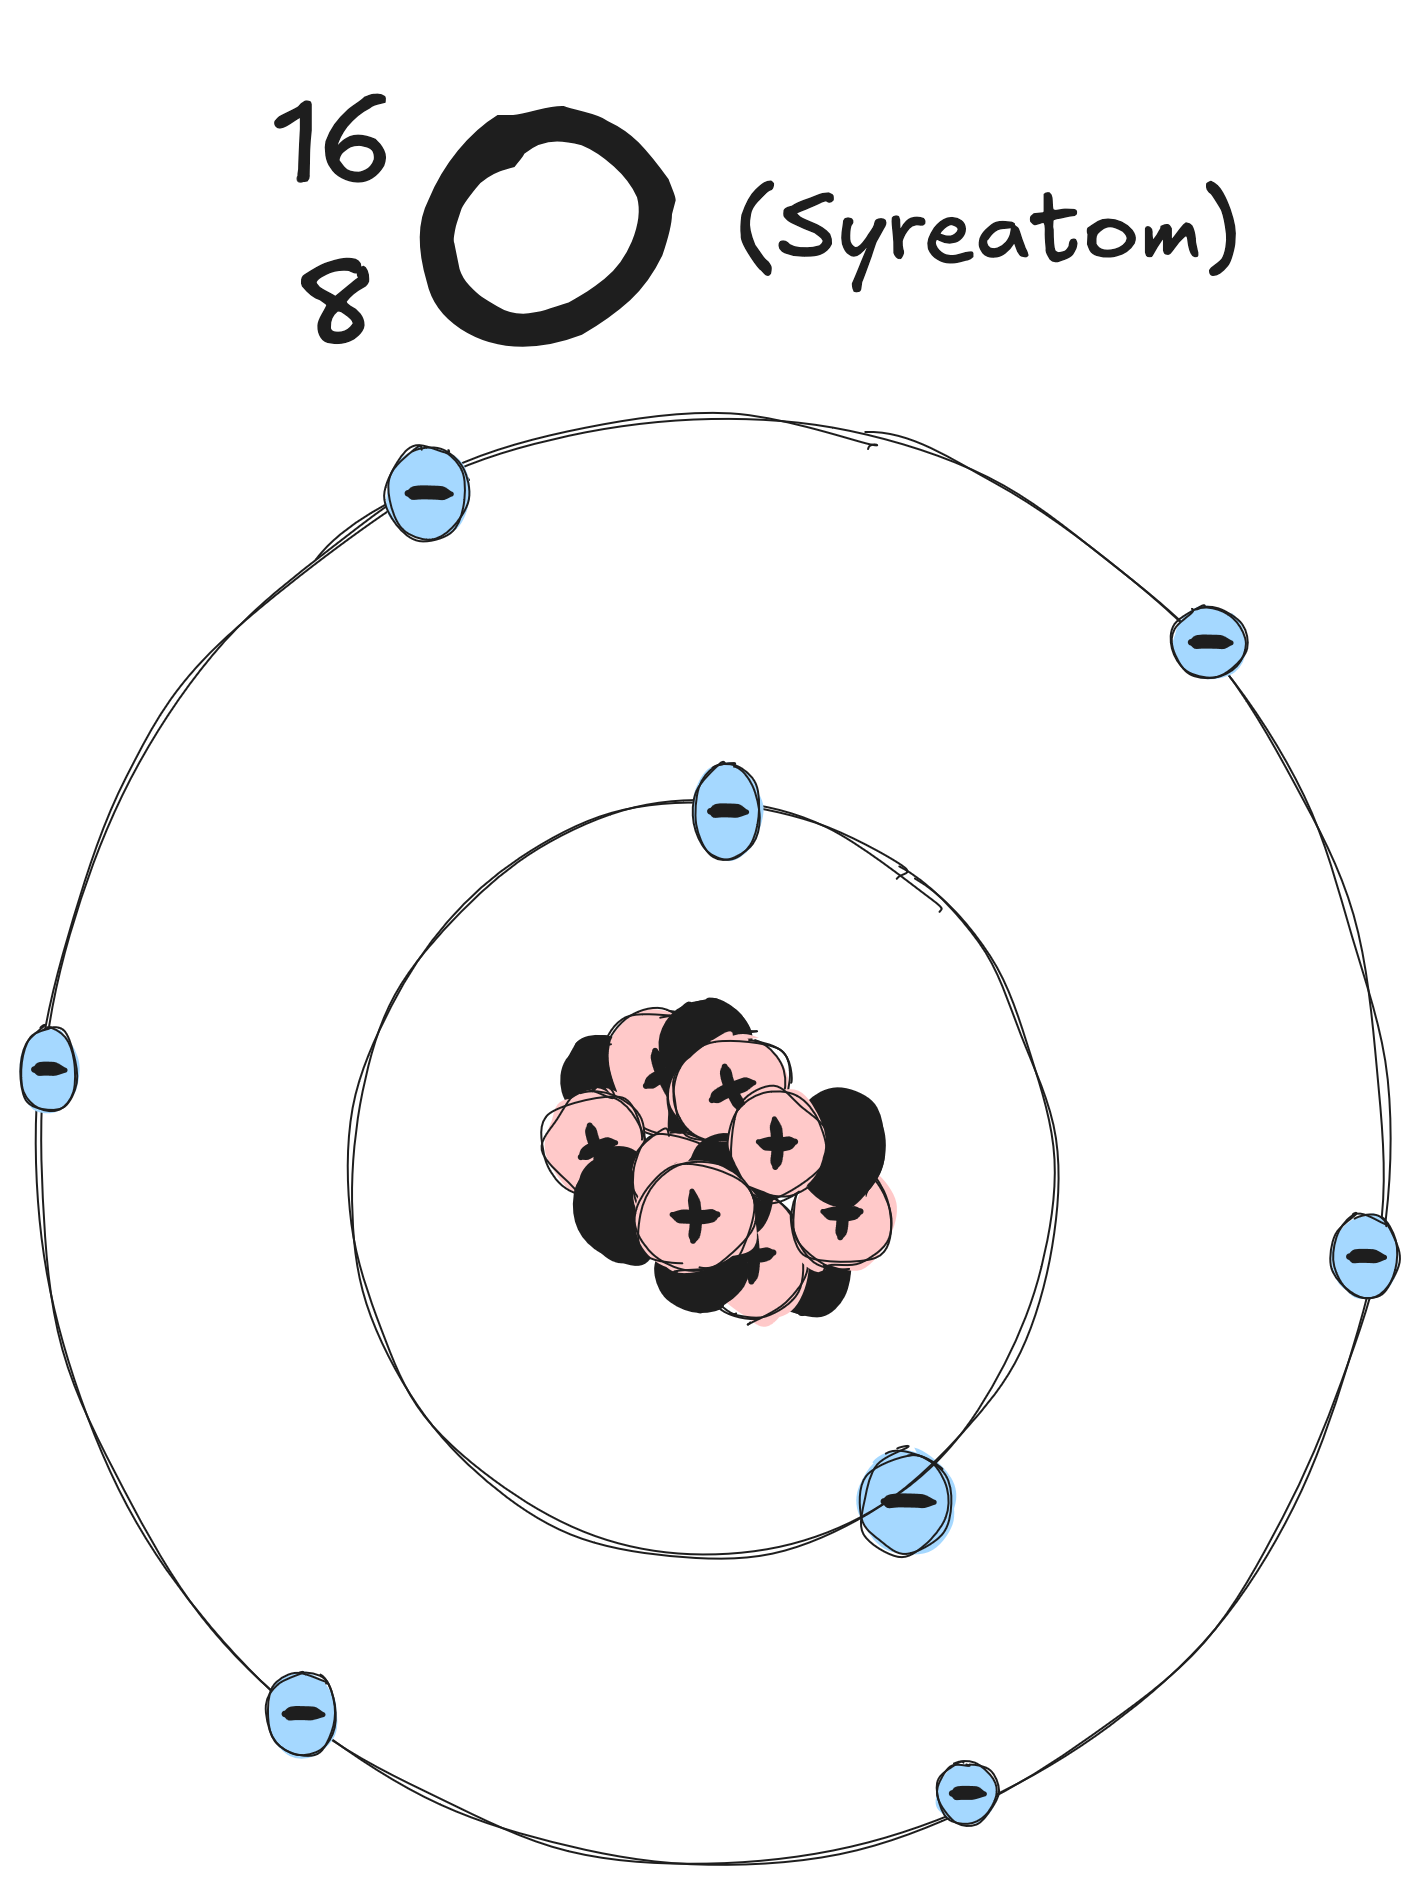
\includegraphics[width=0.25\textwidth]{syre-atom.png}
\end{figure}

\begin{answer}
\textbf{Korrekt svar:} Syre har 6 valenselektroner.

\textbf{Motivering:} Utifrån bilden kan man se att syre har elektroner i det yttersta skalet (valensskalet). Syre har atomnummer 8, vilket betyder att det har 8 elektroner totalt. Elektronerna fördelas i skalen, där de första 2 elektronerna finns i det innersta skalet och de resterande 6 elektronerna finns i valensskalet.

\textbf{Poängbedömning:}
\begin{itemize}
  \item 1 poäng: Korrekt antal valenselektroner (6) med rimlig motivering
  \item 0 poäng: Fel antal valenselektroner eller avsaknad av motivering
\end{itemize}
\end{answer}
\break

\question Vilka av följande molekyler ingår i \textbf{metan-serien}? (\textbf{1 poäng})
\begin{checkboxes}
  \choice \textcolor{blue}{\checkmark} Etan
  \choice Eten
  \choice Butyn
  \choice Propanol
  \choice \textcolor{blue}{\checkmark} Pentan
  \choice Glycerol
\end{checkboxes}
\vspace{5mm}

\begin{answer}
\textbf{Korrekt svar:} Etan och Pentan ingår i metan-serien (alkaner).

\textbf{Förklaring:} Metan-serien (alkaner) är kolväten med enkelbindningar mellan kolatomerna. De har den generella formeln C\textsubscript{n}H\textsubscript{2n+2}.
\begin{itemize}
  \item Etan (C\textsubscript{2}H\textsubscript{6}) - alkan med enkelbindningar
  \item Eten (C\textsubscript{2}H\textsubscript{4}) - alken med dubbelbindning
  \item Butyn (C\textsubscript{4}H\textsubscript{6}) - alkyn med trippelbindning
  \item Propanol (C\textsubscript{3}H\textsubscript{8}O) - alkohol
  \item Pentan (C\textsubscript{5}H\textsubscript{12}) - alkan med enkelbindningar
  \item Glycerol (C\textsubscript{3}H\textsubscript{8}O\textsubscript{3}) - alkohol med tre hydroxylgrupper
\end{itemize}

\textbf{Poängbedömning:}
\begin{itemize}
  \item 1 poäng: Båda rätt markerade och inga felaktiga
  \item 0,5 poäng: En rätt markerad och inga felaktiga
  \item 0 poäng: Felaktiga alternativ markerade
\end{itemize}
\end{answer}
\vspace{5mm}

\question Vad är metanol och vad i dess kemiska struktur gör att det tillhör gruppen? (\textbf{2 poäng})
\vspace{5mm}

\begin{answer}
\textbf{Korrekt svar:} Metanol (CH\textsubscript{3}OH) är den enklaste alkoholen. Det som gör att metanol tillhör gruppen alkoholer är hydroxylgruppen (-OH) som är bunden till en kolatom.

\textbf{Poängbedömning:}
\begin{itemize}
  \item 2 poäng: Korrekt beskrivning av metanol som en alkohol och förklaring att hydroxylgruppen (-OH) gör att den tillhör alkoholgruppen
  \item 1 poäng: Antingen korrekt beskrivning av metanol eller förklaring om hydroxylgruppen
  \item 0 poäng: Felaktig eller ofullständig beskrivning
\end{itemize}
\end{answer}
\vspace{5mm}

\question Vad är \textbf{polyeten} och hur är den uppbyggd? (\textbf{1 poäng})
\vspace{5mm}

\begin{answer}
\textbf{Korrekt svar:} Polyeten är en plast (polymer) som är uppbyggd av många etenmolekyler (monomerer) som har kopplats samman genom polymerisation. När etenmolekylerna kopplas ihop öppnas dubbelbindningarna och bildar långa kedjor av kolatomer med enkelbindningar.

\textbf{Poängbedömning:}
\begin{itemize}
  \item 1 poäng: Beskrivning av polyeten som en polymer uppbyggd av etenmolekyler
  \item 0 poäng: Felaktig eller ofullständig beskrivning
\end{itemize}
\end{answer}
\vspace{5mm}

\question Ge exempel eller förklara följande: (\textbf{2 poäng})
\begin{itemize}
  \item en monosackarid:
  \vspace{5mm}
  \item en disackarid:
  \vspace{5mm}
  \item stärkelse:
  \vspace{5mm}
  \item protein:
\end{itemize}
\vspace{5mm}

\begin{answer}
\textbf{Korrekt svar:}
\begin{itemize}
  \item \textbf{Monosackarid:} Enkel sockerart, t.ex. glukos, fruktos eller galaktos. Kan inte brytas ner till enklare sockerarter.
  \item \textbf{Disackarid:} Består av två monosackarider, t.ex. sackaros (glukos + fruktos), laktos (glukos + galaktos) eller maltos (glukos + glukos).
  \item \textbf{Stärkelse:} En polysackarid uppbyggd av många glukosmolekyler. Fungerar som energilagring i växter.
  \item \textbf{Protein:} Makromolekyler uppbyggda av aminosyror som är sammankopplade med peptidbindningar. Har många funktioner i kroppen, t.ex. som enzymer, transportproteiner, strukturella proteiner.
\end{itemize}

\textbf{Poängbedömning:}
\begin{itemize}
  \item 2 poäng: Korrekt förklaring eller exempel för alla fyra begrepp
  \item 1,5 poäng: Korrekt förklaring eller exempel för tre begrepp
  \item 1 poäng: Korrekt förklaring eller exempel för två begrepp
  \item 0,5 poäng: Korrekt förklaring eller exempel för ett begrepp
  \item 0 poäng: Inga korrekta förklaringar eller exempel
\end{itemize}
\end{answer}
\vspace{5mm}

\question Vad kallas fettsyror som saknar dubbelbindningar? (\textbf{1 poäng})

\begin{answer}
\textbf{Korrekt svar:} Mättade fettsyror.

\textbf{Förklaring:} Mättade fettsyror har endast enkelbindningar mellan kolatomerna och är därmed "mättade" med väteatomer.

\textbf{Poängbedömning:}
\begin{itemize}
  \item 1 poäng: Korrekt svar (mättade fettsyror)
  \item 0 poäng: Felaktigt svar
\end{itemize}
\end{answer}
\break

\question Ange om följande påståenden är sanna eller falska. (\textbf{2 poäng})
\begin{itemize}
  \item De flesta miljögifter är biologiskt nedbrytbara. \textcolor{blue}{(Falskt)}
  \item Mikroplaster kan tas upp av djurplankton i haven. \textcolor{blue}{(Sant)}
  \item Miljögifter är ofta fettlösliga. \textcolor{blue}{(Sant)}
  \item De flesta miljögifter förekommer naturligt i höga koncentrationer i naturen. \textcolor{blue}{(Falskt)}
  \item Koncentrationen av miljögifter är högre i toppkonsumenter än i producenter. \textcolor{blue}{(Sant)}
  \item Plaster bryts snabbt ner i naturen. \textcolor{blue}{(Falskt)}
  \item Plaster kan bidra till spridning av miljögifter i naturen. \textcolor{blue}{(Sant)}
  \item Cocktail-effekten innebär att blandningar av kemikalier alltid är ofarliga. \textcolor{blue}{(Falskt)}
\end{itemize}
\vspace{5mm}

\begin{answer}
\textbf{Korrekta svar:}
\begin{itemize}
  \item De flesta miljögifter är biologiskt nedbrytbara. \textbf{Falskt}
  \item Mikroplaster kan tas upp av djurplankton i haven. \textbf{Sant}
  \item Miljögifter är ofta fettlösliga. \textbf{Sant}
  \item De flesta miljögifter förekommer naturligt i höga koncentrationer i naturen. \textbf{Falskt}
  \item Koncentrationen av miljögifter är högre i toppkonsumenter än i producenter. \textbf{Sant}
  \item Plaster bryts snabbt ner i naturen. \textbf{Falskt}
  \item Plaster kan bidra till spridning av miljögifter i naturen. \textbf{Sant}
  \item Cocktail-effekten innebär att blandningar av kemikalier alltid är ofarliga. \textbf{Falskt}
\end{itemize}

\textbf{Poängbedömning:}
\begin{itemize}
  \item 2 poäng: 7-8 rätta svar
  \item 1,5 poäng: 5-6 rätta svar
  \item 1 poäng: 4 rätta svar
  \item 0,5 poäng: 2-3 rätta svar
  \item 0 poäng: 0-1 rätta svar
\end{itemize}
\end{answer}
\vspace{5mm}

\question Vad händer med kokpunkten för ett \textbf{kolväte} när det blir längre? (\textbf{1 poäng})
\begin{checkboxes}
  \choice \textcolor{blue}{\checkmark} Kokpunkten blir högre.
  \choice Kokpunkten blir lägre.
  \choice Kokpunkten förblir oförändrad.
\end{checkboxes}
\vspace{5mm}  

\begin{answer}
\textbf{Korrekt svar:} Kokpunkten blir högre.

\textbf{Förklaring:} När ett kolväte blir längre (fler kolatomer) ökar de intermolekylära krafterna (van der Waals-krafter) mellan molekylerna, vilket gör att det krävs mer energi för att övergå från vätska till gas. Därför stiger kokpunkten med ökande kolkedjelängd.

\textbf{Poängbedömning:}
\begin{itemize}
  \item 1 poäng: Korrekt svar
  \item 0 poäng: Felaktigt svar
\end{itemize}
\end{answer}
\vspace{5mm}

\question Hur påverkas \textit{struktur- och summaformel} hos \textbf{hexan} om det skulle omvandlas till \textbf{hexen} eller \textbf{hexyn}? Utgå från bilden på hexan nedan. (\textbf{2 poäng})

\begin{figure}[h]
  \centering
  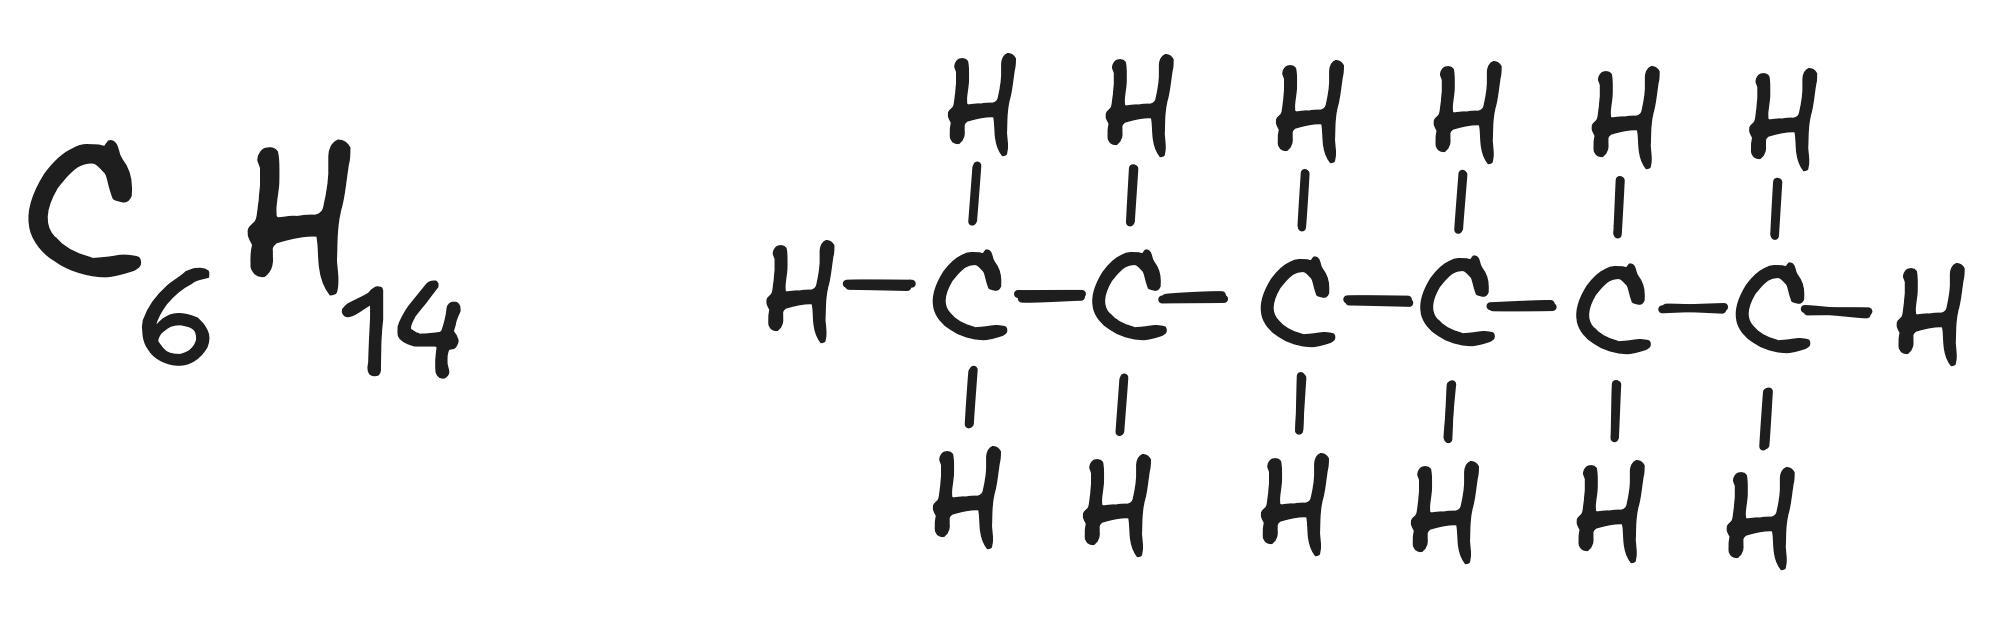
\includegraphics[width=0.4\textwidth]{hexan.png}
\end{figure}
\vspace{5mm}

\begin{answer}
\textbf{Korrekt svar:}

\textbf{Hexan (alkan):}
\begin{itemize}
  \item Summaformel: C\textsubscript{6}H\textsubscript{14}
  \item Strukturformel: Alla bindningar mellan kolatomerna är enkelbindningar
\end{itemize}

\textbf{Hexen (alken):}
\begin{itemize}
  \item Summaformel: C\textsubscript{6}H\textsubscript{12} (två väteatomer färre än hexan)
  \item Strukturformel: En dubbelbindning mellan två kolatomer
\end{itemize}

\textbf{Hexyn (alkyn):}
\begin{itemize}
  \item Summaformel: C\textsubscript{6}H\textsubscript{10} (fyra väteatomer färre än hexan)
  \item Strukturformel: En trippelbindning mellan två kolatomer
\end{itemize}

\textbf{Poängbedömning:}
\begin{itemize}
  \item 2 poäng: Korrekt beskrivning av både summaformel och strukturformel för både hexen och hexyn
  \item 1 poäng: Korrekt beskrivning av antingen summaformel eller strukturformel för både hexen och hexyn, eller korrekt beskrivning av både summa- och strukturformel för endast en av dem
  \item 0 poäng: Felaktiga eller ofullständiga beskrivningar
\end{itemize}
\end{answer}
\break

\question Vad skiljer stärkelse och cellulosa? Vart hittar vi dem och vilken av dem kan vi människor bryta ner? (\textbf{2 poäng})
\vspace{5mm}

\begin{answer}
\textbf{Korrekt svar:}

\textbf{Skillnader:}
\begin{itemize}
  \item Stärkelse och cellulosa är båda polysackarider uppbyggda av glukosmolekyler, men de skiljer sig åt i hur glukosmolekylerna är sammankopplade (olika typer av bindningar).
  \item Stärkelse har alfa-bindningar mellan glukosmolekylerna, medan cellulosa har beta-bindningar.
  \item Stärkelse bildar spiralformade strukturer, medan cellulosa bildar raka kedjor som kan packas tätt och bilda starka fibrer.
\end{itemize}

\textbf{Förekomst:}
\begin{itemize}
  \item Stärkelse finns i växter som energilagring, t.ex. i potatis, ris, pasta och bröd.
  \item Cellulosa finns i växters cellväggar och ger växterna stöd och struktur, t.ex. i trä, bomull och papper.
\end{itemize}

\textbf{Nedbrytning:}
\begin{itemize}
  \item Människor kan bryta ner stärkelse med hjälp av enzymet amylas.
  \item Människor kan inte bryta ner cellulosa eftersom vi saknar enzymet cellulas.
\end{itemize}

\textbf{Poängbedömning:}
\begin{itemize}
  \item 2 poäng: Korrekt beskrivning av skillnader, förekomst och nedbrytning
  \item 1 poäng: Delvis korrekt beskrivning av skillnader, förekomst och nedbrytning
  \item 0 poäng: Felaktig eller ofullständig beskrivning
\end{itemize}
\end{answer}
\vspace{5mm}

\question Resonera kring varför vissa ämnen är miljögifter och hur de kan påverka levande organismer. (\textbf{2 poäng})
\vspace{5mm}

\begin{answer}
\textbf{Korrekt svar:}

\textbf{Varför vissa ämnen är miljögifter:}
\begin{itemize}
  \item De är svårnedbrytbara (persistenta) och kan finnas kvar i miljön under lång tid.
  \item De är ofta fettlösliga och kan därför lagras i fettvävnad hos organismer.
  \item De kan bioackumuleras (ansamlas i organismer) och biomagnifieras (öka i koncentration högre upp i näringskedjan).
  \item De kan transporteras långa sträckor via luft, vatten eller levande organismer.
\end{itemize}

\textbf{Hur miljögifter kan påverka levande organismer:}
\begin{itemize}
  \item Störa hormonsystem (hormonstörande ämnen)
  \item Orsaka cancer eller genetiska skador
  \item Påverka reproduktionsförmågan
  \item Störa immunsystemet
  \item Påverka nervsystemet
  \item Cocktail-effekten: flera miljögifter tillsammans kan ge starkare effekt än summan av de enskilda ämnena
\end{itemize}

\textbf{Poängbedömning:}
\begin{itemize}
  \item 2 poäng: Utförligt resonemang kring både varför ämnen är miljögifter och hur de påverkar organismer
  \item 1 poäng: Grundläggande resonemang kring antingen varför ämnen är miljögifter eller hur de påverkar organismer
  \item 0 poäng: Felaktigt eller ofullständigt resonemang
\end{itemize}
\end{answer}
\vspace{5mm}

\question Förklara hur kolatomens egenskaper gör den speciell för livets kemi (organisk kemi). Använd relevanta begrepp och figurer.(\textbf{3 poäng})
\vspace{5mm}

\begin{answer}
\textbf{Korrekt svar:}

\textbf{Kolatomens speciella egenskaper:}
\begin{itemize}
  \item \textbf{Fyra valenselektroner:} Kol har fyra elektroner i sitt yttersta skal, vilket gör att den kan bilda fyra kovalenta bindningar med andra atomer.
  
  \item \textbf{Förmåga att bilda långa kedjor:} Kol kan binda till andra kolatomer och bilda långa kedjor, förgrenade strukturer eller ringar.
  
  \item \textbf{Olika bindningstyper:} Kol kan bilda enkelbindningar, dubbelbindningar och trippelbindningar med andra kolatomer, vilket ger stor variation i molekylstrukturer.
  
  \item \textbf{Stabilitet:} Kolföreningar är ofta stabila vid normala temperaturer och tryck på jorden.
  
  \item \textbf{Bindningar till andra grundämnen:} Kol kan binda till många andra grundämnen som väte, syre, kväve, svavel och fosfor, vilket är viktigt för att bilda livets byggstenar.
\end{itemize}

\textbf{Betydelse för livets kemi:}
\begin{itemize}
  \item Dessa egenskaper gör att kol kan bilda en enorm mängd olika molekyler med olika funktioner.
  
  \item Kolföreningar utgör grunden för alla levande organismer: kolhydrater, proteiner, lipider och nukleinsyror (DNA, RNA).
  
  \item Möjliggör komplexa strukturer och funktioner som krävs för liv.
\end{itemize}

\textbf{Poängbedömning:}
\begin{itemize}
  \item 3 poäng: Utförlig förklaring av kolatomens egenskaper och deras betydelse för livets kemi, med användning av relevanta begrepp
  
  \item 2 poäng: God förklaring av kolatomens egenskaper och deras betydelse för livets kemi, men med vissa brister eller utan användning av alla relevanta begrepp
  
  \item 1 poäng: Grundläggande förklaring av kolatomens egenskaper eller deras betydelse för livets kemi
  
  \item 0 poäng: Felaktig eller mycket ofullständig förklaring
\end{itemize}
\end{answer}
\vspace{5mm}

\end{questions}

\end{document}
